\documentclass[12pt]{article}

\usepackage{amsmath,amsthm}
\usepackage{newtxtext,newtxmath}
\usepackage{booktabs}
\usepackage{adjustbox}
\usepackage{graphicx}
\graphicspath{{./}{figures/}}
\usepackage[letterpaper,margin=0.9in]{geometry}
\usepackage{xcolor}
\usepackage{float}
\usepackage{caption}
\usepackage{scicite}
\usepackage{url}
\frenchspacing

\renewcommand\refname{References and Notes}
\renewcommand{\thefigure}{S\arabic{figure}}
\renewcommand{\thetable}{S\arabic{table}}
\renewcommand{\thepage}{S\arabic{page}}

\makeatletter
\renewcommand{\fnum@figure}{\textbf{Figure \thefigure}}
\renewcommand{\fnum@table}{\textbf{Table \thetable}}
\makeatother

\begin{document}
\sloppy
\emergencystretch=1.5em

% Lock exact citation numbering 1..45 to match main.pdf identically:
\nocite{daugherty2012rules,enard2016viruses,goldman1994codon,muse1994likelihood,pond2005not,murrell2012detecting,katoh2013mafft,loytynoja2008phylogeny,fletcher2010indelible,jordan2012effects,chavarria2016proteolytic,tsu2021diverse,oliver2009prdm9,patel2016prdm9gene,mcewan2009truncated,braun2015loss,munoz2011orphan,tenthorey2020mutational,kosakovsky2026walrus,methods,kirilenko2023integrating,sawyer2005positive,ito2023a3h,biswal2024stat2,zhao2016irf3,wang2013dpp4,wang2016npc1,lan2020structure,gamble1996crystal,lu2013elob,arragain2024anp32a,li2021rae1,eisenreichova2022ywhaz,guan2011isg15,daczkowski2017isg15,koliopoulos2018trim25,mitchell2012evolution,li2023a3g,guo2014vif,donovan2013oas1,chan2020engineering,jia2009species,mcnatt2009species,elde2009protein,staeheli1986mx}

\begin{center}
\section*{Supplementary Materials for\\ Evolutionary arms races across unalignable mammalian host--virus interfaces}

Sergei~L.~Kosakovsky~Pond$^\ast$, Darren~P.~Martin, Steven~Weaver, and~Anton~Nekrutenko,
corresponding author: spond@temple.edu.
\end{center}

\bigskip
\hrule
\medskip
This PDF file includes Materials and Methods, Supplementary Text (Sections S1 to S3), Figs.~S1 and S2, Tables~S1 to S4, and References and Notes (References \textit{1} to \textit{45} match the main text; References \textit{46} to \textit{61} are cited only in the Supplementary Materials).
\medskip
\hrule
\bigskip

% ============================================================================
\section*{Materials and Methods}
% ============================================================================

\subsection*{Pre-inference objective selection of the 25-locus panel}

To avoid circular selection of classical immune candidates previously curated because of high $dN/dS$ ratios, we implemented an automated pre-inference screen before running any phylogenetic or codon-substitution inference. We queried human Swiss-Prot proteins with canonical length $80 \le L \le 1500$ amino acids annotated with UniProt keyword \texttt{KW-0051} (antiviral defense) or \texttt{KW-0945} (host--virus interaction) \cite{uniprot2023uniprot}. Every candidate protein was intersected against $15,063$ Protein Data Bank (PDB) assemblies containing a human polypeptide chain alongside at least one viral protein chain or nucleic-acid chain at resolution $\le 3.5$\,\AA\ \cite{berman2000protein}. Candidates were ranked solely by experimental resolution, human structural coverage fraction, partner diversity, and documented availability of deep mutational scanning or combinatorial mutagenesis validation \cite{sawyer2004ancient,patel2012antagonism,ng2015filovirus,abraham2010structure,kwong1998structure,lu2013molecular}. Filtering for distinct non-fusion biological assemblies removed crystallographic tag chimeras while preserving native host--virus and protein--nucleic-acid binding pockets across evolutionary diversity. This screen identified $20$ qualifying \texttt{KW-0051} effectors and sensors, $40$ viral entry receptors, and $89$ hijacked cellular host hubs annotated under \texttt{KW-0945} excluding \texttt{KW-0051}.

From those objective ranked lists, we locked a $25$-locus Tier-1 validation panel spanning four orthogonal functional classes prior to running any selection analysis (table~S1). Arm~A consists of $14$ antiviral effectors and innate sensors: \textit{TRIM5}, \textit{MX1}, \textit{APOBEC3G}, \textit{APOBEC3H}, \textit{ISG15}, \textit{SAMHD1}, \textit{STAT2}, \textit{IRF3}, \textit{TRIM25}, \textit{BST2}, \textit{EIF2AK2}, \textit{OAS1}, \textit{MAVS}, and \textit{NLRP1}. Arm~B contains five viral entry receptors with experimentally solved viral glycoprotein co-structures: \textit{ACE2}, \textit{DPP4}, \textit{CD4}, \textit{TFRC}, and \textit{NPC1}. Arm~C supplies the tandem-repeat meiotic regulator \textit{PRDM9}, selected specifically to measure separation between adaptive specificity residues and zinc-finger repeat slippage \cite{patel2016prdm9}. Arm~D provides five hijacked cellular host hubs (\textit{PPIA}, \textit{ELOB}, \textit{ANP32A}, \textit{RAE1}, and \textit{YWHAZ}) that bind HIV-1 Capsid or Vif, Influenza A polymerase, or SARS-CoV-2 viral proteins in PDB co-structures despite performing essential cellular housekeeping functions. Including both cytoplasmic innate sensors and membrane-bound entry receptors alongside replication cofactors targeted by the exact same viral pathogens provides matched internal negative controls for systemic mutation rates, compositional biases, and taxon sampling depth.

\subsection*{Raw unaligned coding sequence curation and atomic contact annotation}

Mammalian orthologous coding DNA sequences (CDS) were curated from TOGA2 whole-genome assemblies \cite{kirilenko2023integrating} supplemented with targeted GenBank orthologues for simian primates (\textit{APOBEC3G} and \textit{APOBEC3H}), bats, carnivores, and cetaceans. Every FASTA dataset contained $50$ to $80$ mammalian taxa ($22$ Simiiformes for primate-restricted \textit{APOBEC3G}) with valid DNA nucleotides and an intact human reference matching canonical UniProt at $1.000$ amino-acid identity. Unlike standard selection pipelines that discard interrupted genes prior to alignment, curated inputs retained native frameshifts and internal stop codons verbatim across seven documented mammalian pseudogenes. Those loci comprise feline \textit{TRIM5} (\textit{Felis catus}), four delphinid \textit{MX1} orthologues (\textit{Delphinus delphis}, \textit{Globicephala melas}, \textit{Orcinus orca}, and \textit{Pseudorca crassidens}), and both canid \textit{PRDM9} orthologues (\textit{Canis lupus} and \textit{Canis aureus}). Retaining uninterrupted wild-type flanking sequence alongside frameshifted exons permits direct likelihood comparison between background purifying constraints and relaxed pseudogene substitution regimes within one phylogenomic run. This unified input structure eliminates separate curatorial branches for pseudogenized versus intact orthologues.

Structural and functional annotations were fixed prior to inspecting selection calls across all $25$ loci. For the $19$ non-fusion PDB co-structures (PDB accessions listed in table~S2) \cite{schwefel2014samhd1,li2023vif,abraham2010structure,kwong1998structure,ng2015filovirus}, atomic mmCIF or PDB coordinates were aligned directly to the canonical human sequence. For every resolved human residue, we computed minimum heavy-atom Euclidean distance $d_{\min}$ across all non-hydrogen atom pairs connecting the human polypeptide to any viral protein or nucleic-acid partner chain. Residues were partitioned into direct contacts ($d_{\min} \le 4.5$\,\AA), proximal shells ($4.5 < d_{\min} \le 8.0$\,\AA), buried cores ($d_{\min} > 8.0$\,\AA), and PDB-unmodeled regions. For \textit{SAMHD1} (PDB 4CC9), where only the carboxyl-terminal degron helix is resolved, non-contact comparisons evaluated $>4.5$\,\AA\ residues. For the six Arm~A loci without full-length viral co-structures (\textit{TRIM5}, \textit{MX1}, \textit{BST2}, \textit{EIF2AK2}, \textit{MAVS}, and \textit{NLRP1}), functional loop and viral cleavage-tripwire windows were taken verbatim from published mutagenesis scans \cite{tenthorey2020mutational,mitchell2012evolution,mcnatt2009species,elde2009protein,patel2012antagonism,tsu2021diverse}. For \textit{PRDM9}, canonical \texttt{C-X2-C-X12-H-X3-H} zinc-finger motifs were indexed automatically to separate DNA major-groove specificity positions ($-1$, $+2$, $+3$, $+6$ relative to $\alpha$-helix start) from zinc-coordinating cysteine and histidine ligands and structural framework sites.

\subsection*{Unified statistical alignment, reticulation, and biophysical inference}

All $25$ raw unaligned CDS datasets were executed end-to-end with WALRUS in HyPhy 3 using flags \texttt{-u --coevolution --keep-pseudogenes} \cite{kosakovsky2026walrus}. As detailed previously \cite{kosakovsky2026walrus}, WALRUS performs reading-frame repair and pseudogene admission directly on unaligned FASTA input, optimizes an Inside--Outside pair hidden Markov model over codon homology posteriors, and screens segmental topological incongruence via an Ohmic Wheatstone conductance network \cite{pond2006gard}. On that statistical homology ensemble, the engine tests directional GC3 base-composition drift, evaluates gene-wide episodic diversifying selection under BUSTED-E \cite{selberg2024busted}, and scores branch-level RELAX intensity ($k$) and loss-of-function Bayes factors \cite{wertheim2015relax,smith2015less}. Downstream site likelihoods jointly estimate diversifying selection, amino-acid exchangeability toggling, alignment-artifact demotion, and epistatic coevolution pairs across up to $25$ top-ranked mutational linkages per locus. Site innovation calls combined diversifying, two-state toggle, or convergent classes passing Benjamini--Hochberg false-discovery control ($q \le 0.10$) or MEME episodic support ($q \le 0.10$). Demoted alignment artifacts were archived verbatim rather than silently deleted, which maintains exact per-locus artifact bookkeeping.

On each converged WALRUS alignment and phylogeny, property-informed selection was evaluated with \texttt{hyphy3 sprime} under the five-property biophysical basis (\texttt{--property-set 5PROP}) using conservative Empirical Bayes Ridge regularization (\texttt{--shrinkage 0.5}). The five orthogonal physicochemical axes comprise isoelectric point, Chou--Fasman $\alpha$-helix propensity, Chou--Fasman $\beta$-sheet propensity, Kyte--Doolittle hydrophobicity, and side-chain volume in \AA$^3$. Regularization shrinks poorly sampled amino-acid exchange vectors back toward site-neutral evolutionary rates so that rare substitutions cannot inflate property weights. Under this conservative parameterization, strict two-stage S-PRIME reprogramming requires both site-wide omnibus likelihood ratio significance ($\mathrm{BH}\ q \le 0.10$) and individual property Holm--Bonferroni significance ($p_{\mathrm{adj}} \le 0.10$). Marginal property calls relax the omnibus gate while retaining Holm--Bonferroni $p_{\mathrm{adj}} \le 0.10$, separating signed property change ($\lambda < 0$) from property conservation ($\lambda > 0$). For baseline comparisons on \textit{TRIM5} and \textit{PRDM9}, intact sequences were translated, aligned with progressive MAFFT v7 \cite{katoh2013mafft}, back-translated to codons, and analyzed under standard site-level FEL and MEME \cite{pond2005not,murrell2012detecting}.

\subsection*{Pan-mammalian TOGA2 cohort construction and statistical tests}

To evaluate proteome-wide evolutionary generality, we analyzed $7,045$ completed mammalian orthogroup summaries generated uniformly under WALRUS from the TOGA2 mammalian alignment archive \cite{kirilenko2023integrating,kosakovsky2026walrus}. Deduplicating transcripts to one canonical isoform per official human gene symbol and enforcing $n_{\text{taxa}} \ge 25$ and length $\ge 50$ codons yielded $49$ antiviral effectors and sensors (\texttt{KW-0051}), $179$ hijacked cellular host hubs (\texttt{KW-0945} excluding \texttt{KW-0051}), and $6,817$ background mammalian genes (table~S4). All enrichment ratios across discrete structural classes were evaluated with Fisher's exact tests using one-sided within-complex tests matching pre-registered contact-enrichment hypotheses and two-sided between-class comparisons. Within-gene paired contact-versus-core differences across the $13$ conflict PDB complexes used two-sided Wilcoxon signed-rank tests, and unpaired cross-gene or cross-proteome contrasts used two-sided Mann--Whitney $U$ tests. To verify that Tier-2 proteome differences were not confounded by sequence length or alignment depth, we fitted ordinary least-squares regressions incorporating group indicators alongside $\log(n_{\text{taxa}})$ and $\log(n_{\text{codons}})$ covariates across all loci. Those adjusted linear regressions confirmed persistent elevation of episodic selection ($+4.82\%$, $p = 1.3 \times 10^{-4}$), insertion--deletion gap density ($+3.69\%$, $p = 0.0014$), and amino-acid toggling ($+10.29\%$, $p = 7.4 \times 10^{-4}$) in antiviral genes relative to hubs (table~S4).

% ============================================================================
\section*{Supplementary Text}
% ============================================================================

\subsection*{Section S1: Progressive alignment distortions versus joint homology ensembles}

Progressive multiple sequence aligners assume homogeneous branching processes without length-changing frameshifts, causing severe positional distortions across rapidly remodeling immune loci. On \textit{TRIM5}, omitting feline \textit{TRIM5} and running MAFFT stretched the alignment to $650$ codons and generated $56$ nominal episodic calls under standard MEME ($p \le 0.05$, reduced to $1$ after multiple-testing correction), primarily concentrated near ambiguous loop boundaries (fig.~S2A). Joint homology modeling admitted all $67$ mammals into a compact $595$-codon ensemble with mean column posterior certainty $0.955$, removed $6$ rigid-alignment false positives, and maintained significant enrichment inside the experimentally validated PRYSPRY v1--v4 capsid-binding loops ($\mathrm{OR} = 2.09$, $p = 0.00392$). Across \textit{PRDM9}, repeat-array copy variation caused progressive alignment to stretch to $1,467$ codons and misalign $16$ zinc-finger register columns (fig.~S2A), whereas joint ensemble inference condensed the locus to $1,334$ columns, eliminated $48$ spurious calls, and isolated diversifying selection at DNA-contacting residues ($75.0\%$ versus $2.1\%$ structural zinc ligands). Extending across all $25$ Tier-1 loci, joint ensemble modeling removed $279$ alignment-induced false-positive calls (led by $51$ in \textit{NLRP1}, $48$ in \textit{PRDM9}, $24$ in \textit{STAT2}, $21$ in \textit{IRF3}, and $20$ in \textit{OAS1}; table~S1).

\subsection*{Section S2: Reticulate Ohmic Wheatstone bridges and base-composition drift}

When multigene defense families or paralogous domains exchange short tracts between diverging lineages, conditioning codon substitution inference on a single global tree can attribute shared ancestral blocks to parallel positive selection \cite{pond2006gard,kosakovsky2021contrast}. Across the $25$ Tier-1 loci, conductance scanning detected $393$ putative bridge candidates, $10$ of which passed permutation and segmental likelihood thresholds ($\Delta \ln L = 11.20$ to $67.34$, conductance $0.842$ to $1.416$, permutation $p = 0.0020$ to $0.0040$; fig.~S2B and table~S3). Prior to optimizing site selection tests, WALRUS dynamically routed each supported tract through a local subtree prune-and-regraft topology. The strongest routed exchange spanned codons $498$--$623$ across laurasiatherian internal branches in \textit{MX1} ($\Delta \ln L = 67.34$), followed by a carnivoran--camelid tract in \textit{NLRP1} (\textit{Meles meles} to \textit{Camelus bactrianus}, codons $2102$--$2203$, $\Delta \ln L = 47.23$). Supported tracts also linked simian \textit{NPC1} ($\Delta \ln L = 32.32$), bat and dolphin \textit{IRF3} (\textit{Pipistrellus kuhlii} to \textit{Aethalodelphis obliquidens}, $\Delta \ln L = 29.32$), cetacean \textit{OAS1} (\textit{Mesoplodon mirus} to \textit{Phocoena phocoena}, $\Delta \ln L = 20.80$), \textit{TRIM5}, \textit{MAVS}, and \textit{APOBEC3H}. In addition, third-codon-position compositional audits revealed significant base-composition heterogeneity in $16$ of $25$ Tier-1 loci (led by \textit{RAE1}, $p = 1.83 \times 10^{-168}$; \textit{NLRP1}, $p = 1.99 \times 10^{-161}$; \textit{NPC1}, $p = 2.87 \times 10^{-111}$; and \textit{EIF2AK2}, $p = 2.77 \times 10^{-81}$; table~S1).

\subsection*{Section S3: Unsupervised loss-of-function profiles and short-branch caveats}

Admitting raw coding sequences without stop-codon pre-filtering enabled unsupervised phylogenetic screening for relaxed selection and lineage-specific gene loss across $96$ flagged branches in Tier~1 (table~S1). All seven repaired pseudogenes produced strong branch-level Bayes factors, led by canid \textit{PRDM9} (\textit{Canis aureus}, $p = 8.67 \times 10^{-95}$; \textit{Canis lupus}, $p = 1.75 \times 10^{-19}$) alongside an independent degu relaxation branch (\textit{Octodon degus}, $p = 1.14 \times 10^{-16}$, $k = 0.605$). Unsupervised screening also uncovered parallel pseudogenization or relaxation in lineages lacking curated stop annotations. Notable examples include murine \textit{MX1} ($p = 2.68 \times 10^{-9}$, $k = 0.532$), chiropteran \textit{TRIM5} (\textit{Miniopterus fuliginosus}, $p = 5.77 \times 10^{-9}$, $k = 0.078$), cetacean \textit{OAS1} (\textit{Aethalodelphis obliquidens}, $p = 1.39 \times 10^{-17}$; \textit{Leucopleurus acutus}, $p = 4.32 \times 10^{-15}$), carnivoran \textit{NLRP1} (\textit{Ursus arctos}, $p = 7.62 \times 10^{-23}$), and bat and pangolin \textit{IRF3} (\textit{Myotis lucifugus}, $p = 1.66 \times 10^{-92}$; \textit{Manis javanica}, $p = 2.99 \times 10^{-27}$). By contrast, isolated short-branch flags across hijacked hubs (\textit{ELOB} in \textit{Condylura cristata}, $p = 2.23 \times 10^{-40}$, $k = 0.445$, and \textit{Otolemur garnettii}, $p = 1.62 \times 10^{-23}$, $k = 0.061$; alongside \textit{PPIA}, \textit{ANP32A}, \textit{RAE1}, and \textit{YWHAZ}) coincide with $0.0\%$ strict S-PRIME reprogramming, indicating processed retrocopies or assembly edge artifacts rather than adaptive host remodeling.

\clearpage

% ============================================================================
\section*{Supplementary Figures}
% ============================================================================

\begin{figure}[H]
\centering
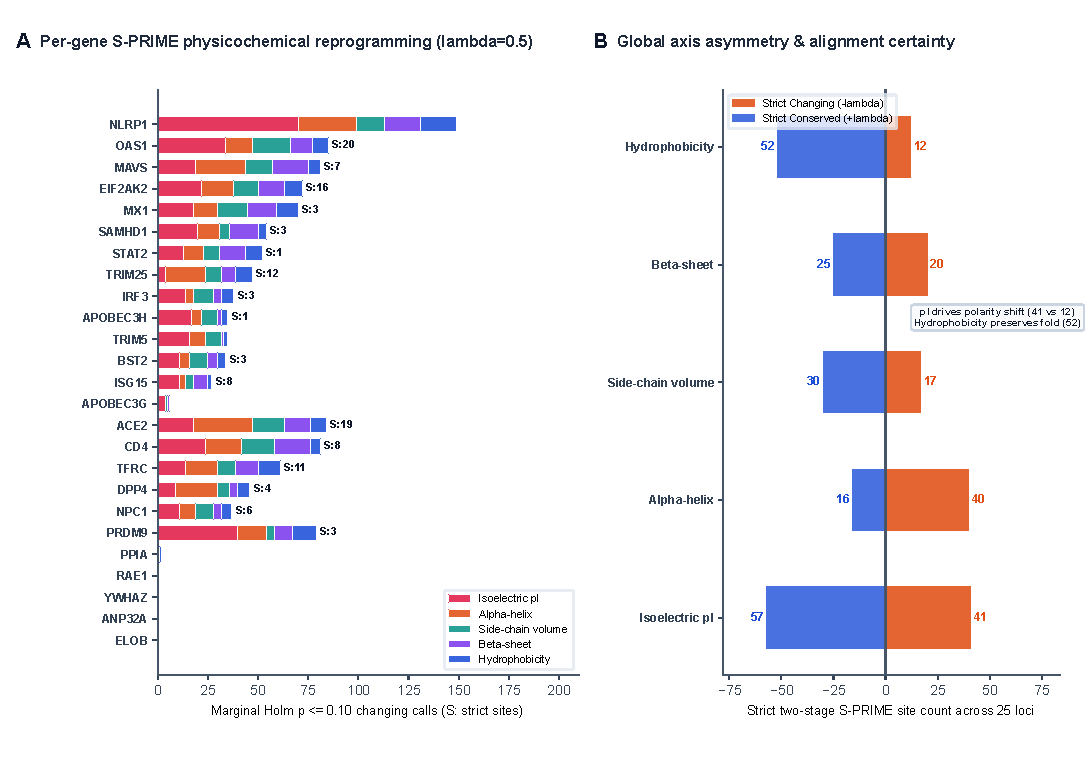
\includegraphics[width=0.98\textwidth,height=0.68\textheight,keepaspectratio]{fig_s1_property_and_error_audit.pdf}
\caption{Biophysical selection architecture across all 25 Tier-1 loci under conservative Empirical Bayes Ridge S-PRIME ($\lambda = 0.5$). (A) Stacked per-locus counts of marginal Holm-adjusted ($p_{\mathrm{adj}} \le 0.10$) property-changing calls colored across five physicochemical dimensions. Right-hand labels report total strict two-stage sites (omnibus $q \le 0.10$ and $p_{\mathrm{adj}} \le 0.10$), topped by \textit{OAS1} ($12$ strict isoelectric-point sites out of $34$ marginal), \textit{ISG15} ($6$ of $11$), \textit{EIF2AK2} ($6$ of $22$), and \textit{PRDM9} ($3$ of $40$). (B) Global symmetry breaking across the five biophysical properties compares strict changing sites ($\lambda < 0$, orange) against strict conserved sites ($\lambda > 0$, blue). Isoelectric point acts as the primary adaptive switching axis ($41$ strict changing sites), whereas hydrophobicity stabilizes core folding ($52$ strict conserved versus $12$ changing).}
\label{fig:s1_prime}
\end{figure}

\begin{figure}[H]
\centering
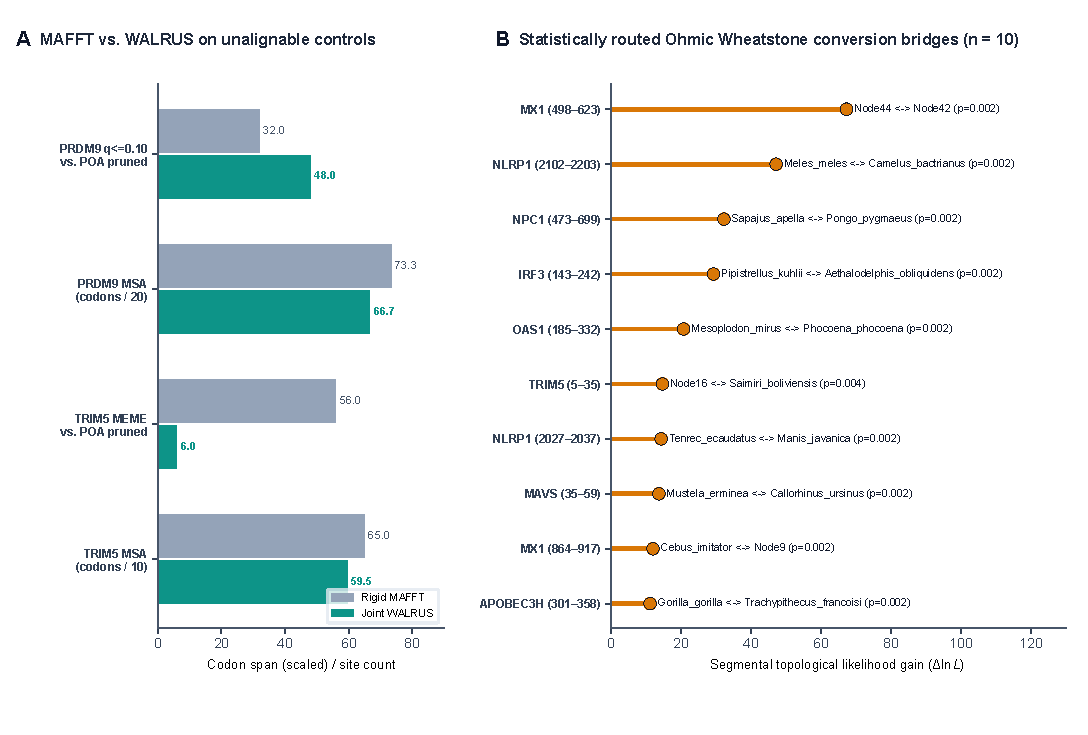
\includegraphics[width=0.98\textwidth,height=0.68\textheight,keepaspectratio]{fig_s2_legacy_and_wheatstone.pdf}
\caption{Progressive alignment artifacts and statistically routed gene-conversion tracts. (A) Head-to-head comparison between progressive MAFFT codon alignment paired with standard MEME selection inference (gray) and unified WALRUS joint modeling (teal) on \textit{TRIM5} ($595$ versus $650$ codons, $6$ artifacts pruned) and \textit{PRDM9} ($1,334$ versus $1,467$ codons, $48$ artifacts pruned), reporting scaled alignment lengths and episodic call counts. Across all $25$ loci, statistical homology awareness prevented $279$ false-positive selection calls. (B) Cleveland profile across all $10$ statistically supported Ohmic Wheatstone gene-conversion bridges routed onto alternative topologies prior to selection testing ($\Delta \ln L = 11.20$ to $67.34$, permutation $p = 0.0020$ to $0.0040$). The largest routed tracts occur in laurasiatherian \textit{MX1} ($\Delta \ln L = 67.34$) and carnivoran--camelid \textit{NLRP1} ($\Delta \ln L = 47.23$).}
\label{fig:s2_wheatstone}
\end{figure}

\clearpage

% ============================================================================
\section*{Supplementary Tables}
% ============================================================================

\begin{table}[htbp]
\centering
\caption{Complete evolutionary ledger across all 25 pre-registered Tier-1 mammalian loci evaluated from unaligned coding sequences with pseudogene rescue and conservative Ridge S-PRIME shrinkage ($\lambda = 0.5$).}
\label{tab:s1_tier1_atlas}
\footnotesize
\setlength{\tabcolsep}{3.6pt}
\begin{adjustbox}{max width=\textwidth}
\begin{tabular}{@{}l r r r r r r r r r@{}}
\toprule
Gene & Taxa & Ref/MSA & Ins. & Gap\% & Sel.\% & BUSTED-E $p$ & Art. & pI (M/S) & LoF (Ps) / Coev \\
\midrule
\multicolumn{10}{@{}l}{\textit{Antiviral effectors and innate sensors ($n = 14$)}} \\
\quad \texttt{TRIM5} & 67 & 493/595 & 92 & 16.4 & 21.9 & $1.000$ & 6 & 16/0 & 1 (+1) / 25 \\
\quad \texttt{MX1} & 80 & 662/955 & 121 & 31.1 & 15.1 & $1.3\times 10^{-12}$ & 7 & 18/0 & 10 (+4) / 25 \\
\quad \texttt{APOBEC3G} & 22 & 384/411 & 20 & 7.0 & 33.6 & $9.4\times 10^{-49}$ & 0 & 4/0 & 1 / 15 \\
\quad \texttt{APOBEC3H} & 69 & 200/368 & 136 & 45.4 & 16.0 & $3.1\times 10^{-41}$ & 11 & 17/0 & 5 / 7 \\
\quad \texttt{ISG15} & 72 & 165/241 & 74 & 30.5 & 21.2 & $0.0095$ & 12 & 11/6 & 0 / 2 \\
\quad \texttt{SAMHD1} & 72 & 626/731 & 93 & 15.0 & 23.7 & $2.9\times 10^{-17}$ & 4 & 20/1 & 6 / 25 \\
\quad \texttt{STAT2} & 72 & 851/1187 & 229 & 28.1 & 22.1 & $0.066$ & 24 & 13/1 & 7 / 25 \\
\quad \texttt{IRF3} & 72 & 427/604 & 107 & 29.5 & 18.2 & $1.0\times 10^{-4}$ & 21 & 14/2 & 3 / 25 \\
\quad \texttt{TRIM25} & 72 & 630/720 & 61 & 12.4 & 34.2 & $2.0\times 10^{-7}$ & 8 & 4/2 & 5 / 24 \\
\quad \texttt{BST2} & 72 & 180/289 & 89 & 37.9 & 18.0 & $5.3\times 10^{-19}$ & 11 & 11/1 & 2 / 0 \\
\quad \texttt{EIF2AK2} & 72 & 551/765 & 171 & 28.5 & 26.7 & $1.9\times 10^{-58}$ & 7 & 22/6 & 3 / 9 \\
\quad \texttt{OAS1} & 72 & 400/613 & 179 & 38.6 & 23.6 & $1.3\times 10^{-42}$ & 20 & 34/12 & 3 / 12 \\
\quad \texttt{MAVS} & 72 & 540/893 & 235 & 40.6 & 16.8 & $9.1\times 10^{-24}$ & 16 & 19/0 & 6 / 25 \\
\quad \texttt{NLRP1} & 55 & 1473/2231 & 534 & 36.0 & 17.1 & $2.9\times 10^{-34}$ & 51 & 70/0 & 3 / 25 \\
\midrule
\multicolumn{10}{@{}l}{\textit{Viral entry receptors ($n = 5$)}} \\
\quad \texttt{ACE2} & 72 & 805/843 & 35 & 4.9 & 31.6 & $1.7\times 10^{-39}$ & 3 & 18/3 & 1 / 25 \\
\quad \texttt{DPP4} & 72 & 766/775 & 8 & 1.2 & 29.6 & $1.9\times 10^{-15}$ & 0 & 9/0 & 1 / 23 \\
\quad \texttt{CD4} & 72 & 458/608 & 106 & 24.7 & 27.5 & $3.8\times 10^{-34}$ & 6 & 24/0 & 2 / 0 \\
\quad \texttt{TFRC} & 72 & 760/803 & 25 & 4.9 & 30.4 & $2.0\times 10^{-6}$ & 0 & 14/2 & 5 / 25 \\
\quad \texttt{NPC1} & 55 & 1278/1474 & 35 & 13.5 & 18.1 & $1.7\times 10^{-4}$ & 2 & 11/2 & 6 / 25 \\
\midrule
\multicolumn{10}{@{}l}{\textit{Tandem-repeat meiotic benchmark ($n = 1$)}} \\
\quad \texttt{PRDM9} & 50 & 894/1334 & 319 & 37.1 & 13.1 & $4.2\times 10^{-35}$ & 48 & 40/3 & 6 (+2) / 25 \\
\midrule
\multicolumn{10}{@{}l}{\textit{Hijacked cellular host hubs ($n = 5$)}} \\
\quad \texttt{PPIA} & 72 & 165/224 & 24 & 26.6 & 6.7 & $0.115$ & 6 & 0/0 & 6 / 0 \\
\quad \texttt{ELOB} & 72 & 118/199 & 67 & 37.5 & 3.0 & $1.000$ & 14 & 0/0 & 3 / 25 \\
\quad \texttt{ANP32A} & 72 & 249/268 & 15 & 7.3 & 12.3 & $1.000$ & 2 & 0/0 & 6 / 2 \\
\quad \texttt{RAE1} & 72 & 368/461 & 0 & 19.9 & 0.7 & $1.000$ & 0 & 1/0 & 4 / 0 \\
\quad \texttt{YWHAZ} & 72 & 245/245 & 0 & 0.5 & 0.0 & $1.000$ & 0 & 0/0 & 1 / 0 \\
\bottomrule
\end{tabular}
\end{adjustbox}
\end{table}

\begin{table}[htbp]
\centering
\caption{Atomic heavy-atom partner contact ($d_{\min} \le 4.5$\,\AA) versus buried scaffold ($>8.0$\,\AA) enrichment across 19 experimental PDB co-structures. For SAMHD1 4CC9, non-contact compares $>4.5$\,\AA\ residues.}
\label{tab:s2_pdb_atomic}
\footnotesize
\setlength{\tabcolsep}{3.8pt}
\begin{adjustbox}{max width=\textwidth}
\begin{tabular}{@{}l l r r r r r@{}}
\toprule
Gene & Partner complex (PDB) & Contact ($\le 4.5$\,\AA) & Core ($>8.0$\,\AA) & OR & Fisher $p$ & Gap$_{\le 4.5}$ / Gap$_{\text{unmod}}$ \\
\midrule
\multicolumn{7}{@{}l}{\textit{Conflict complexes: antiviral effectors and sensors ($n = 8$)}} \\
\quad \texttt{APOBEC3G} & HIV-1 Vif (8CX0) & 6/13 (46.1\%) & 117/340 (34.4\%) & 1.63$\times$ & $0.277$ & 0.0\% / 30.1\% \\
\quad \texttt{APOBEC3H} & HIV-1 Vif (8FVI) & 7/13 (53.9\%) & 32/144 (22.2\%) & 4.08$\times$ & $0.019$ & 1.0\% / 69.6\% \\
\quad \texttt{ISG15} & FluB NS1B / PLpro (3SDL, 5TL6) & 11/42 (26.2\%) & 23/68 (33.8\%) & 0.69$\times$ & $0.854$ & 3.5\% / 29.6\% \\
\quad \texttt{SAMHD1} & SIV Vpx (4CC9) & 6/13 (46.1\%) & 5/6 (83.3\%) & 0.17$\times$ & $0.983$ & 8.1\% / 2.1\% \\
\quad \texttt{STAT2} & Dengue NS5 (8T12) & 15/36 (41.7\%) & 99/390 (25.4\%) & 2.10$\times$ & $0.031$ & 3.6\% / 6.6\% \\
\quad \texttt{IRF3} & Rotavirus NSP1 (5JER) & 9/18 (50.0\%) & 42/192 (21.9\%) & 3.57$\times$ & $0.012$ & 0.9\% / 2.6\% \\
\quad \texttt{TRIM25} & FluA NS1 (5NT1) & 11/20 (55.0\%) & 56/125 (44.8\%) & 1.51$\times$ & $0.271$ & 0.0\% / 3.2\% \\
\quad \texttt{OAS1} & dsRNA (4IG8) & 14/37 (37.8\%) & 89/253 (35.2\%) & 1.12$\times$ & $0.442$ & 3.8\% / 62.8\% \\
\midrule
\multicolumn{7}{@{}l}{\textit{Conflict complexes: viral entry receptors ($n = 5$)}} \\
\quad \texttt{ACE2} & SARS-CoV-2 RBD (6M0J) & 10/21 (47.6\%) & 159/545 (29.2\%) & 2.21$\times$ & $0.062$ & 1.4\% / 0.2\% \\
\quad \texttt{DPP4} & MERS-CoV RBD (4L72) & 13/23 (56.5\%) & 185/674 (27.4\%) & 3.44$\times$ & $0.0038$ & 0.5\% / 1.6\% \\
\quad \texttt{CD4} & HIV-1 gp120 (1GC1) & 11/24 (45.8\%) & 54/138 (39.1\%) & 1.32$\times$ & $0.344$ & 7.9\% / 3.6\% \\
\quad \texttt{TFRC} & Machupo GP1 (3KAS) & 8/24 (33.3\%) & 181/583 (31.1\%) & 1.11$\times$ & $0.485$ & 1.7\% / 1.9\% \\
\quad \texttt{NPC1} & Ebola GP (5F1B) & 6/15 (40.0\%) & 26/191 (13.6\%) & 4.23$\times$ & $0.016$ & 0.0\% / 0.9\% \\
\midrule
\multicolumn{7}{@{}l}{\textit{Tandem-repeat DNA complex ($n = 1$)}} \\
\quad \texttt{PRDM9} & Hotspot DNA (5EGB) & 20/50 (40.0\%) & 2/24 (8.3\%) & 7.33$\times$ & $0.0040$ & 17.1\% / 11.4\% \\
\midrule
\multicolumn{7}{@{}l}{\textit{Hijacked cellular hub controls ($n = 5$)}} \\
\quad \texttt{PPIA} & HIV-1 CA (1AK4) & 1/20 (5.0\%) & 14/119 (11.8\%) & 0.40$\times$ & $0.915$ & 0.2\% / --- \\
\quad \texttt{ELOB} & HIV-1 Vif (2MA9, 4N9F) & 1/5 (20.0\%) & 4/107 (3.7\%) & 6.44$\times$ & $0.208$ & 1.7\% / --- \\
\quad \texttt{ANP32A} & FluA Pol (8RN0) & 3/36 (8.3\%) & 8/81 (9.9\%) & 0.83$\times$ & $0.719$ & 0.2\% / 5.8\% \\
\quad \texttt{RAE1} & SARS-CoV-2 Orf6 (7VPG) & 0/23 (0.0\%) & 1/273 (0.4\%) & 0.00$\times$ & $1.000$ & 0.0\% / 0.2\% \\
\quad \texttt{YWHAZ} & SARS-CoV-2 N (7ZIT) & 0/18 (0.0\%) & 0/179 (0.0\%) & --- & $1.000$ & 0.8\% / 1.4\% \\
\midrule
Pooled conflict ($n=13$) & Within-complex ($\le 4.5$\,\AA\ vs.\ core) & 127/299 (42.5\%) & 1063/3643 (29.2\%) & 1.79$\times$ & $1.9\times 10^{-6}$ & 2.5\% / 16.5\% \\
Pooled hubs ($n=5$) & Controls ($\le 4.5$\,\AA\ vs.\ core) & 5/102 (4.9\%) & 27/759 (3.6\%) & 1.40$\times$ & $0.326$ & 0.6\% / 2.5\% \\
\bottomrule
\end{tabular}
\end{adjustbox}
\end{table}

\begin{table}[htbp]
\centering
\caption{All 10 statistically routed Ohmic Wheatstone gene-conversion tracts detected across the 25 Tier-1 loci before site selection evaluation.}
\label{tab:s3_wheatstone}
\footnotesize
\setlength{\tabcolsep}{4.5pt}
\begin{adjustbox}{max width=\textwidth}
\begin{tabular}{@{}l l l r r r r@{}}
\toprule
Gene & Donor/source node & Recipient/target node & Codon interval & $\Delta \ln L$ & Conductance & Perm.\ $p$ \\
\midrule
\texttt{MX1} & \texttt{Node44} & \texttt{Node42} & 498--623 & 67.34 & 1.303 & 0.0020 \\
\texttt{NLRP1} & \texttt{Meles\_meles} & \texttt{Camelus\_bactrianus} & 2102--2203 & 47.23 & 1.127 & 0.0020 \\
\texttt{NPC1} & \texttt{Sapajus\_apella} & \texttt{Pongo\_pygmaeus} & 473--699 & 32.32 & 1.227 & 0.0020 \\
\texttt{IRF3} & \texttt{Pipistrellus\_kuhlii} & \texttt{Aethalodelphis\_obliquidens} & 143--242 & 29.32 & 1.256 & 0.0020 \\
\texttt{OAS1} & \texttt{Mesoplodon\_mirus} & \texttt{Phocoena\_phocoena} & 185--332 & 20.80 & 1.416 & 0.0020 \\
\texttt{TRIM5} & \texttt{Node16} & \texttt{Saimiri\_boliviensis} & 5--35 & 14.72 & 0.842 & 0.0040 \\
\texttt{NLRP1} & \texttt{Tenrec\_ecaudatus} & \texttt{Manis\_javanica} & 2027--2037 & 14.37 & 1.087 & 0.0020 \\
\texttt{MAVS} & \texttt{Mustela\_erminea} & \texttt{Callorhinus\_ursinus} & 35--59 & 13.74 & 0.991 & 0.0020 \\
\texttt{MX1} & \texttt{Cebus\_imitator} & \texttt{Node9} & 864--917 & 12.03 & 1.389 & 0.0020 \\
\texttt{APOBEC3H} & \texttt{Gorilla\_gorilla} & \texttt{Trachypithecus\_francoisi} & 301--358 & 11.20 & 1.175 & 0.0020 \\
\bottomrule
\end{tabular}
\end{adjustbox}
\end{table}

\begin{table}[htbp]
\centering
\caption{Pan-mammalian TOGA2 proteome divergence across 7,045 canonical orthogroups and covariate-adjusted ordinary least-squares estimates controlling for $\log(\text{taxa})$ and $\log(\text{codons})$.}
\label{tab:s4_tier2_toga2}
\footnotesize
\setlength{\tabcolsep}{4.5pt}
\begin{adjustbox}{max width=\textwidth}
\begin{tabular}{@{}l r r r r r@{}}
\toprule
Comparison / metric & Value ($n$ or $\beta$) & SE & Test statistic & Two-sided $p$ & Notes \\
\midrule
Antiviral vs.\ hubs: episodic site \% (OLS) & $+4.82\%$ & 1.24 & $t=3.90$ & $1.3\times 10^{-4}$ & $n=49$ vs.\ $179$ \\
Antiviral vs.\ hubs: gap density \% (OLS) & $+3.69\%$ & 1.14 & $t=3.23$ & $0.0014$ & $n=49$ vs.\ $179$ \\
Antiviral vs.\ hubs: toggle/conv \% (OLS) & $+10.29\%$ & 3.01 & $t=3.42$ & $7.4\times 10^{-4}$ & $n=49$ vs.\ $179$ \\
Antiviral vs.\ background: episodic \% (OLS) & $+4.50\%$ & 0.91 & $t=4.94$ & $7.9\times 10^{-7}$ & $n=49$ vs.\ $6,817$ \\
Antiviral vs.\ background: gap \% (OLS) & $+2.19\%$ & 1.17 & $t=1.87$ & $0.062$ & $n=49$ vs.\ $6,817$ \\
Antiviral vs.\ hubs: BUSTED-E \% (Fisher) & $69.39\%$ vs.\ $39.11\%$ & --- & --- & $1.5\times 10^{-4}$ & $34/49$ vs.\ $70/179$ \\
Hijacked hubs higher taxon retention (MWU) & $839$ vs.\ $441$ taxa & --- & --- & $1.9\times 10^{-7}$ & Median conserved taxa \\
\bottomrule
\end{tabular}
\end{adjustbox}
\end{table}


\clearpage

\bibliography{references}
\bibliographystyle{sciencemag}

\end{document}
